\documentclass[t,aspectratio=1610]{beamer}

\usepackage{bxcjkjatype}
\usepackage{listings}
\usepackage{tikz}
\newcounter{row}
\newcounter{col}

\newcommand\setrow[9]{
  \setcounter{col}{1}
  \foreach \n in {#1, #2, #3, #4, #5, #6, #7, #8, #9} {
    \edef\x{\value{col} - 0.5}
    \edef\y{9.5 - \value{row}}
    \node[anchor=center] at (\x, \y) {\n};
    \stepcounter{col}
  }
  \stepcounter{row}
}

\usetheme{default}
\beamertemplatenavigationsymbolsempty\setbeamersize{
    text margin left=0.75cm,
    text margin right=0.75cm
}

% Title
\setbeamerfont{title}{size=\LARGE, 
                      series=\bfseries,
                      family=\rmfamily}
\setbeamercolor{title}{fg=blue!70!black}
\setbeamertemplate{frametitle}{
    \nointerlineskip\;
    \begin{beamercolorbox}[sep=.1ex,
                           wd=\paperwidth,
                           leftskip=0.5cm,
                           rightskip=0pt]{frametitle}
        \usebeamerfont{frametitle}
        \usebeamercolor[fg]{frametitle}
        \\
        \hfill
        \insertfrmetitle\;
        \strut\;
    \end{beamercolorbox}
}
% Alerted text
\setbeamerfont{alerted text}{shape=\itshape,
                             series=\bfseries}
\setbeamercolor{alerted text}{fg=black!90}
% Itemize
\setbeamercolor{itemize item}{fg=black!90}
\setbeamercolor{itemize subitem}{fg=black!90}
\setbeamertemplate{itemize item}[circle]
\setbeamertemplate{itemize subitem}[triangle]
% Blocks
\setbeamercolor{block body example}{fg=black!90,
                                    bg=black!10}
\setbeamercolor{block title example}{fg=white,
                                     bg=blue!30!black!30}
\setbeamertemplate{blocks}[shadow=true]

\newcommand{\sidesplit}[4][0.25]{%
    \centering
    \begin{minipage}{#1\textwidth}
    \resizebox{\textwidth}{!}{#2}
    \end{minipage}
    \hfill
    \begin{minipage}{#1\textwidth}
    \resizebox{\textwidth}{!}{#3}
    \end{minipage}
    \hfill
    \begin{minipage}{#1\textwidth}
    \resizebox{\textwidth}{!}{#4}
    \end{minipage}
}


\title{Courses @ USI (CUSI)}
\subtitle{Mobile \& Wearable Computing}
\author{Bevilacqua Joey \\ Lagrasta Federico \\ Rodolfo Masera Tommaso}
\institute{Universit\`a della Svizzera Italiana\\ Faculty of Informatics\\ \href{http://www.unisi.ch}{www.unisi.ch}}
\date{Nov 4, 2021}

\begin{document}
{
% Slide 1: Title slide
% - Name of app and of group members

%\usebackgroundtemplate{\includegraphics[width=1\paperwidth, height=1\paperheight]{screamc}}
\begin{frame}
\maketitle
\end{frame}
}

{
% Slide 2: Motivation slide
% - What is the problem your app is supposed to solve?
% - Why do you expect it to be useful?
% - What’s wrong with existing solutions (if applicable)

\begin{frame}
\textbf{Motivation} \\

\begin{itemize}
\item The problem the app is supposed to solve
\item Why we expect it to be usiful
\item What's wrong with existing solutions
\end{itemize}
\end{frame}
}

{
% Slide 3: Project slide
% - Describe how you plan to implemented your app
\begin{frame}
\textbf{Motivation} \\

\begin{enumerate}
\item Step 1
\item Step 2
\item Step 3
\end{enumerate}
\end{frame}
}

{
% Slide 4: Storyboard slide
% - Add the storyboard of your app
\begin{frame}
\textbf{Storyboard} \\

% \vspace{-0.6em}
\centerline{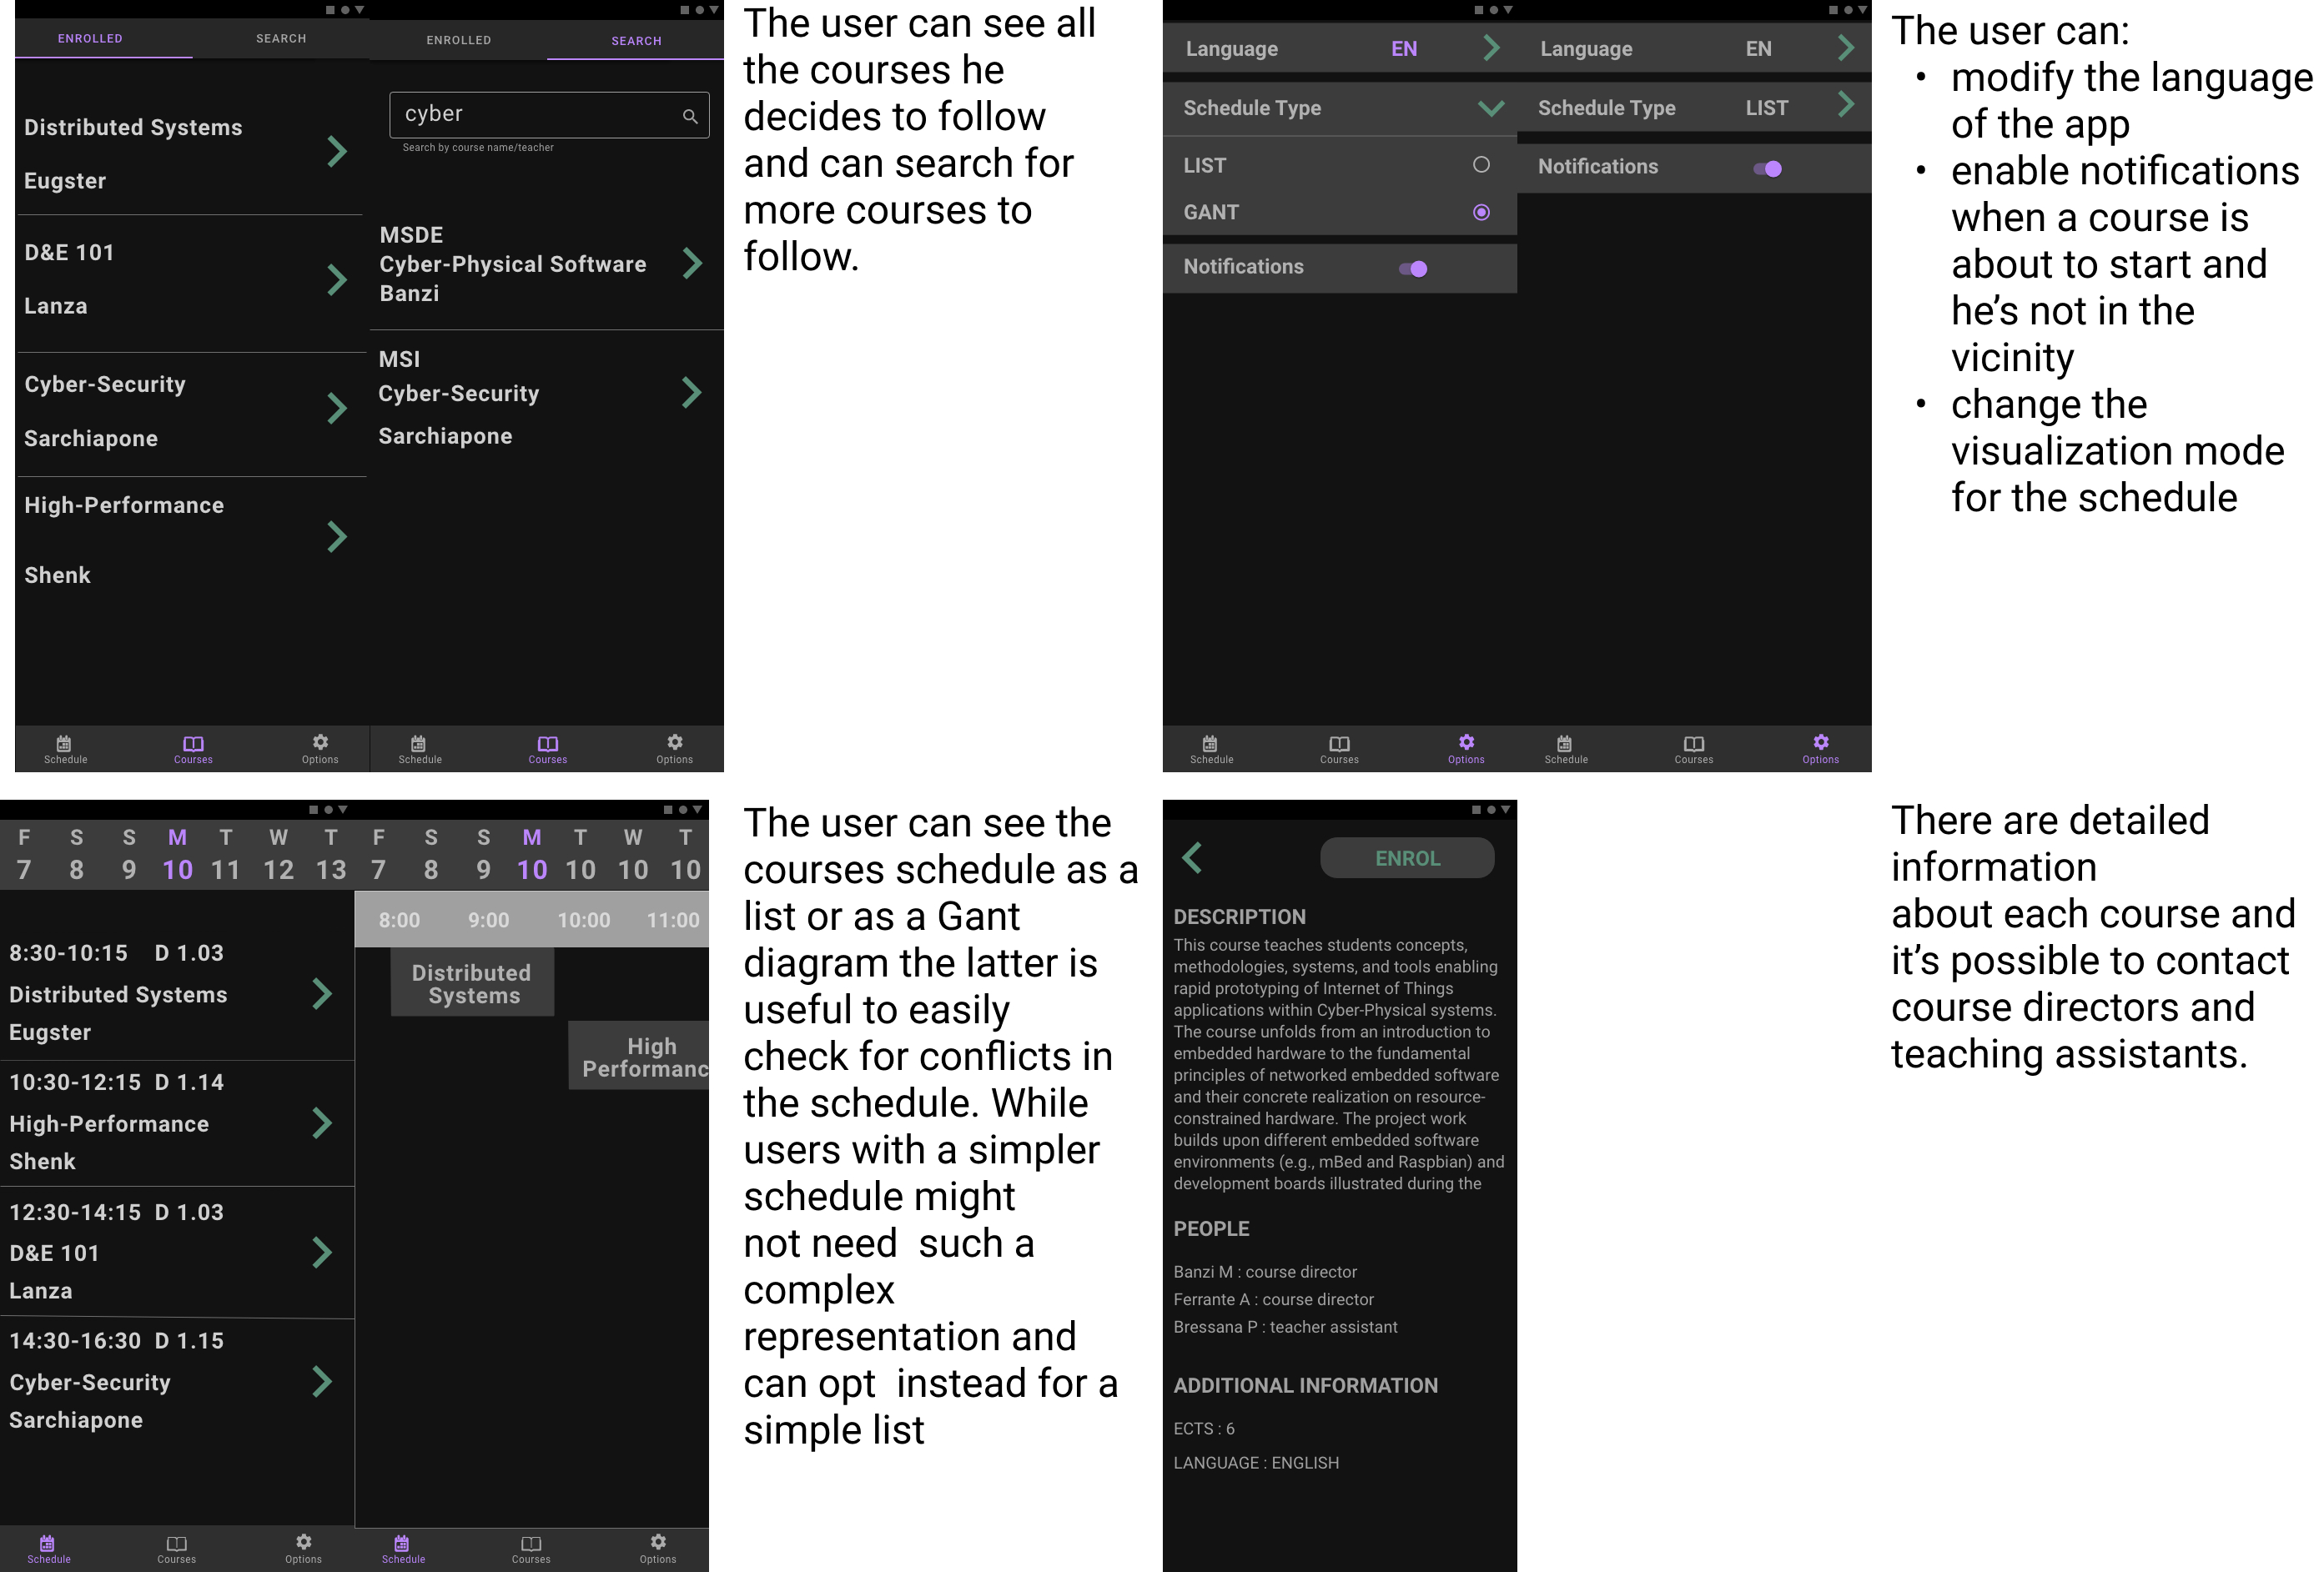
\includegraphics[scale=0.13]{storyboard.jpg}}
\end{frame}
}

{
% Slide 5: Thank you slide
% - Tank you https://youtu.be/usWfJ0EJLB0?t=1047

\begin{frame}
\textbf{Thanks} \\

% \vspace{-0.6em}
% \centerline{\includegraphics[scale=0.25]{tanks.png}}
\end{frame}
}
\end{document}
